\section{Performance test}

\subsection{Parallel matrix multiplication algorithms}

We will use the matrix multiplication as algorithm to test the performance of \Kotlin and \Go coroutine implementations. There will be three different versions of the algorithm:

\begin{itemize}
	\item \textbf{FAN}:\\
	Uses 2 channels: one to distribute the cells to be computed (\texttt{taskChannel}), the other to collect the partial results (\texttt{resultChannel}); thanks to the \texttt{fan}, all the workers wait on the same channel and send their result on the other. A coordinator is in charge to open the channels, launch the workers, distribute the work, collect the results and finally close the channels, automatically notifying the end of the computation.
	
	\item \textbf{COORDINATOR}:\\
	Requires a coordinator \textit{server} like the previous, but a greater amount of channels: one channel shared  by the workers to notify their availability (\texttt{requestWorkChannel}), one channel the workers can use to notify their termination (\texttt{ackChannel}), one channel to send the partial results (\texttt{resultChannel}), and one channel for each worker the coordinator uses to send the cell to be computed (\texttt{workerChannels[]}). 
	
	The matrices are still on the shared memory and their reference is passed to the workers. The coordinator has to listen both of the \texttt{requestChannel} and the 	\texttt{resultChannel} to react to the availability of a worker or to the computation of a partial result: when all the cells are computed, the coordinator notifies each worker channel, then wait for their termination and returns the final result.
	
	\item \textbf{PURE}\\
	This algorithm is the same of the previous, but the matrices are not in the shared memory anymore, so the coordinator send the row and the column the worker has to use to produce the result for the requested cell.
	
	This is a pure implementation of a message-passing algorithm, without any shared memory but only using channels and messages.
\end{itemize}

\begin{center}
	\begin{tabular}{|>{\raggedright\arraybackslash}p{4cm}|>{\raggedright\arraybackslash}p{4cm}|>{\raggedright\arraybackslash}p{4cm}|}
		\hline
		\textbf{Algorithm} & \textbf{Shared Memory Usage} & \textbf{Number of Channels} \\
		\hline
		\textbf{FAN} & Input Matrices & 2 \\
		\hline
		\textbf{COORDINATOR} & Input Matrices & 3 + $N_{WORKERS}$ \\
		\hline
		\textbf{PURE} & None & 3 + $N_{WORKERS}$ \\
		\hline
	\end{tabular}
\end{center}

While \Kotlin offers a solid \textit{object-oriented} paradigm, \Go has only a minimal support for it: while for the first language we have one interface in its file and the implementation in their own files, all the \Go code is enclosed in a single file following the language's conventions:

\begin{center}
	\begin{tabular}{|>{\raggedright\arraybackslash}p{3cm}|>{\raggedright\arraybackslash}p{9cm}|}
		\hline
		\textbf{Language} & \textbf{Implementations} \\
		\hline
		\Kotlin & 
		\begin{tabular}[t]{@{}l@{}}
			\href{https://github.com/LM-96/Activity-Project-Operating-Systems-M-/blob/main/code/kotlin/unibo.apos.examples/src/main/kotlin/unibo/apos/matrix/product/MatrixProduct.kt}{\texttt{MatrixProduct.kt}} \\
			\href{https://github.com/LM-96/Activity-Project-Operating-Systems-M-/blob/main/code/kotlin/unibo.apos.examples/src/main/kotlin/unibo/apos/matrix/product/impl/FanChanneledMatrixProductImpl.kt}{\texttt{FanChanneledMatrixProductImpl.kt}} \\
			\href{https://github.com/LM-96/Activity-Project-Operating-Systems-M-/blob/main/code/kotlin/unibo.apos.examples/src/main/kotlin/unibo/apos/matrix/product/impl/CoordinatorChanneledMatrixProductImpl.kt}{\texttt{CoordinatorChanneledMatrixProductImpl.kt}} \\
			\href{https://github.com/LM-96/Activity-Project-Operating-Systems-M-/blob/main/code/kotlin/unibo.apos.examples/src/main/kotlin/unibo/apos/matrix/product/impl/PureChanneledMatrixProductImpl.kt}{\texttt{PureChanneledMatrixProductImpl.kt}} \\
		\end{tabular} \\
		\hline
		\Go & 
		\href{https://github.com/LM-96/Activity-Project-Operating-Systems-M-/blob/main/code/go/matrix/matrix.go}{\texttt{matrix.go}} \\
		\hline
	\end{tabular}
\end{center}

\subsection{Main and launchers for performance analysis}

In order to use the algorithm that have just been presented, we need two main application:
\begin{center}
	\begin{tabular}{|>{\raggedright\arraybackslash}p{3cm}|>{\raggedright\arraybackslash}p{9cm}|}
		\hline
		\textbf{Language} & \textbf{Implementations} \\
		\hline
		\Kotlin & 
		\begin{tabular}[t]{@{}l@{}}
			\href{https://github.com/LM-96/Activity-Project-Operating-Systems-M-/blob/main/code/kotlin/unibo.apos.examples/src/main/kotlin/unibo/apos/KAposMatrixApp.kt}{\texttt{KAposMatrixApp.kt}} \\
		\end{tabular} \\
		\hline
		\Go & 
		\href{https://github.com/LM-96/Activity-Project-Operating-Systems-M-/blob/main/code/go/main.go}{\texttt{main.go}} \\
		\hline
	\end{tabular}
\end{center}

Both of the \texttt{main} functions, accept that series of parameters in order to \textbf{perform the computation of the product of two matrices with the specified size, using the given number of coroutines}.
In addition, the programs have been implemented with the possibility to store the results in a \texttt{csv}, specifying a file to go in append mode.

Notice that:
\begin{itemize}
	\item the\uline{ \Kotlin} application must be \uline{built using \href{https://gradle.org/}{\texttt{Gradle}}}, for example via the task \texttt{distZip} that creates a convenient launcher to execute the jar
	\item  the \uline{\Go} application has to be \uline{compiled using \href{https://go.dev/doc/tutorial/compile-install}{\texttt{go build}}}
\end{itemize}

Once the executable are created, they can be invoked using the arguments specified in the following table:

\begin{center}
	\begin{tabular}{|>{\raggedright\arraybackslash}p{3cm}|>{\raggedright\arraybackslash}p{3cm}|>{\raggedright\arraybackslash}p{7cm}|}
		\hline
		\textbf{Option} & \textbf{Default Value} & \textbf{Description} \\
		\hline
		\texttt{-s, --size} & 3 & Size of the matrices (NxN) \\
		\hline
		\texttt{-c, --coroutines} & 4 & Number of coroutines to use \\
		\hline
		\texttt{-o, --output} & \texttt{false} & Store results in CSV file \\
		\hline
		\texttt{-f, --file} & \texttt{null} & CSV filename for storing results \\
		\hline
		\texttt{-r, --repeat} & 1 & Number of times to repeat the calculation \\
		\hline
		\texttt{-l, --log} & false & Enable detailed logging \\
		\hline
		\texttt{-m, --mode} & \texttt{COORDINATOR} & Concurrency mode: \texttt{COORDINATOR}, \texttt{FAN}, or \texttt{PURE} \\
		\hline
	\end{tabular}
\end{center}

\textbf{The argument \texttt{-r} allows to repeat the multiplication for the specified number of times with the given parameters}: each run is then associated to the same \textbf{workspace}.
A workspace is \uline{a set of execution with the same parameters} and it's used in order to perform average logic and enhance the precision of the analysis.

To easily produce the executables and launch them at once with suitable sets of values for the matrix size and the workers, a convenient launcher for \texttt{Linux} has been developed at \href{https://github.com/LM-96/Activity-Project-Operating-Systems-M-/blob/main/code/launcher.sh}{\texttt{launcher.sh}}.

That launcher executes two kind of analysys:

\begin{itemize}
	\item \textbf{FIXED SIZE}\\
	The \uline{size of the matrices is fixed} while \uline{the number of the workers is increased} execution by execution.
	
	\item \textbf{FIXED WORKER}\\
	The \uline{number of the workers is fixed} but \uline{the size of the matrix varies} execution by execution.
\end{itemize}

Each set of $(size, workers)$ is executed for 10 times. This way, then the \texttt{csv} is produced, just the average of the execution times of the repetitions of the same set will be considered.

\subsection{Native compilation for \Kotlin}

\subsubsection{\Kotlin Native}

Kotlin supports \href{https://kotlinlang.org/docs/native-overview.html}{\textbf{native compilation}} realized from the same \texttt{Jetbrains} by involving \href{https://llvm.org/}{LLVM}.

We want to add also \texttt{Kotlin Native} in the comparison to analyze the difference between \texttt{Kotlin JVM} and \Go.

Notice that when \Kotlin is configured to work in the native mode (see \href{https://github.com/LM-96/Activity-Project-Operating-Systems-M-/blob/main/code/kotlin-native/build.gradle.kts}{\texttt{build.gradle.kts}}), the set of usable library is reduced and the \textbf{Java} standard libraries are not supported anymore (even the \texttt{Java IO/NIO}). For this reason, some modifications to the existing \Kotlin code were needed: you can find here the \href{https://github.com/LM-96/Activity-Project-Operating-Systems-M-/tree/main/code/kotlin-native}{\texttt{kotlin-native}} project with the right configuration and a thinner code that allows the compilation.

A convenient launcher as also be developed to launch the native compilation and the execution with the same parameters of the launcher shown in the paragraph above: \href{https://github.com/LM-96/Activity-Project-Operating-Systems-M-/blob/main/code/launcher_ktntv.sh}{\texttt{launcher\_ktntv.sh}}

\subsubsection{\Kotlin compiled via \texttt{GraalVM}}

Java itself supports native compilation thanks to an external and advanced \texttt{JVM} with innovative technologies that supports a process called \href{https://www.graalvm.org/latest/reference-manual/native-image/}{\textit{ahead-of-time Native Image compilation}}.

We will not go deep into the details of this project, but we are going to use it to test this other way to compile native \Kotlin code. Notice that, differently from the previous solution, this one is not developed from \texttt{Jetbrains}, but from an external community of developers. Indeed, \texttt{GraalVM} was initially developed for \texttt{Java} but, since \Kotlin compiles itself \texttt{Java}, it is also compatible without problems.

The configuration of \texttt{GraalVM}'s compilation does not involve complex processes than modifying the \href{https://github.com/LM-96/Activity-Project-Operating-Systems-M-/blob/main/code/kotlin/unibo.apos.examples/build.gradle}{\texttt{build.gradle}} with the proper plugin conveniently configured.

The setup is carefully explained at \href{https://graalvm.github.io/native-build-tools/latest/gradle-plugin.html}{this page} but, as done for the others, we developed a launcher also for the \texttt{GraalVM} version at \href{https://github.com/LM-96/Activity-Project-Operating-Systems-M-/blob/main/code/launcher_graal.sh}{\texttt{launcher\_graal.sh}}.

\subsection{Overview of the considered versions and plotting}

Based on what has been presented, the following table summarizes all the algorithms and the version of the languages we are going to use to perform the analysis:

\begin{center}
	\begin{tabular}{|>{\raggedright\arraybackslash}p{3cm}|>{\raggedright\arraybackslash}p{4cm}|>{\raggedright\arraybackslash}p{3cm}|>{\raggedright\arraybackslash}p{3cm}|}
		\hline
		\textbf{} & \textbf{COORDINATOR} & \textbf{FAN} & \textbf{PURE} \\
		\hline
		\textbf{Kotlin} & \texttt{kt\_coordinator} & \texttt{kt\_fan} & \texttt{kt\_pure} \\
		\hline
		\textbf{Kotlin Native} & \texttt{kt\_ntv\_coordinator} & \texttt{kt\_ntv\_fan} & \texttt{kt\_ntv\_pure} \\
		\hline
		\textbf{Kotlin Graal} & \texttt{kt\_graal\_coordinator} & \texttt{kt\_graal\_fan} & \texttt{kt\_graal\_pure} \\
		\hline
		\textbf{Go} & \texttt{go\_coordinator} & \texttt{go\_fan} & \texttt{go\_pure} \\
		\hline
	\end{tabular}
\end{center}

The results of the executions will be placed into proper csv:
\begin{itemize}
		\item \href{https://github.com/LM-96/Activity-Project-Operating-Systems-M-/blob/main/code/benchmark_results/fixed_size_sel.csv}{\texttt{fixed\_size\_sel.csv}} for the results of the \textit{fixed size} analysis
		
		\item 
		\href{https://github.com/LM-96/Activity-Project-Operating-Systems-M-/blob/main/code/benchmark_results/fixed_workers_sel.csv}{\texttt{fixed\_workers\_sel.csv}} for the results of the \textit{fixed workers} analysis
\end{itemize}

Another component \href{https://github.com/LM-96/Activity-Project-Operating-Systems-M-/tree/main/code/server}{\texttt{server}} has been developed in order to accept the \texttt{csv} files and produce the graph we are going to show.

Again, we developed a script to easily call the server to produce the graphs: \href{https://github.com/LM-96/Activity-Project-Operating-Systems-M-/blob/main/code/graphs.sh}{\texttt{graphs.sh}}

\subsection{All-in-one graphs}

\begin{figure}[H]
	\centering
	\begin{minipage}{0.7\textwidth}
		\centering
		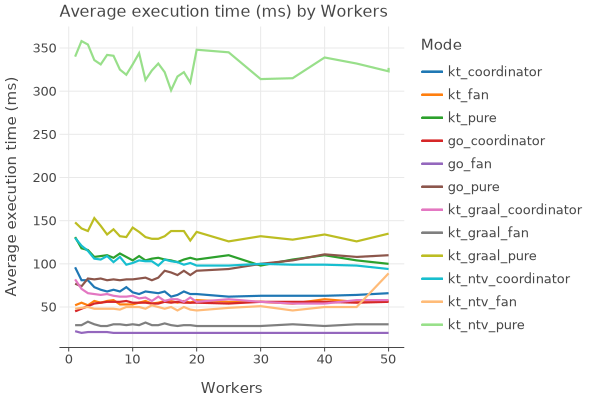
\includegraphics[width=\textwidth]{img/graphs/fixed_size_all}
		\caption{Fixed Size Analysis}
	\end{minipage}\hfill
	\begin{minipage}{0.25\textwidth}
		The graph clearly shows a huge variety of performance between the different variants.  We can see that \Go \texttt{FAN} has the best performance, followed by \Kotlin Graal at the same variant.
		Without any doubt, the worse is \Kotlin Native in pure mode, meaning that pure message-passing communication could not be optimized in the native compiled sources.
	\end{minipage}
\end{figure}

\begin{figure}[H]
	\centering
	\begin{minipage}{0.7\textwidth}
		\centering
		\includegraphics[width=\textwidth]{img/graphs/fixed_workers_all}
		\caption{Fixed Worker Analysis}
	\end{minipage}\hfill
	\begin{minipage}{0.25\textwidth}
		Also this graph seems to confirm the impressions above, with \Kotlin Native having the worst performance. Anyway, \Kotlin Native in the \texttt{FAN} mode performs slightly well, but \Go confirms to be less time-consuming both in the \texttt{FAN} and \texttt{COORDINATOR} modes. Anyway, the \texttt{PURE} modes have the worst times while the \texttt{FAN} have the bests.
	\end{minipage}
\end{figure}

\subsection{Graphs by modes}

\subsubsection{Fixed size}

\begin{figure}[H]
	\centering
	\begin{minipage}{0.7\textwidth}
		\centering
		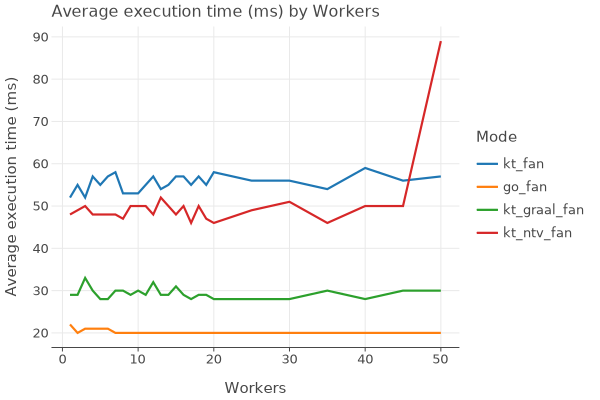
\includegraphics[width=\textwidth]{img/graphs/fixed_size_fan}
		\caption{Fixed Size Analysis \texttt{FAN}}
	\end{minipage}\hfill
	\begin{minipage}{0.25\textwidth}
		\Go and \Kotlin \texttt{Graal} still are the bests while \Kotlin Native initially seems to be winning on \texttt{JVM}, but it definitively looses with a huge number of workers. In addition, \Go seems to resist really well to the increase of the workers, keeping the execution time almost constant and demonstrating a huge ability to handle a significant amount of concurrent units.
	\end{minipage}
\end{figure}

\begin{figure}[H]
	\centering
	\begin{minipage}{0.7\textwidth}
		\centering
		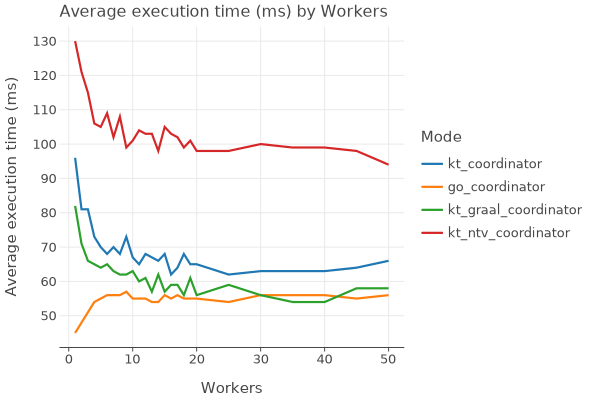
\includegraphics[width=\textwidth]{img/graphs/fixed_size_coordinator}
		\caption{Fixed Size Analysis  \texttt{COORDINATOR}}
	\end{minipage}\hfill
	\begin{minipage}{0.25\textwidth}
		\Go still confirms as the one that takes less time while \Kotlin Native keeps being the worst.
		\texttt{GraalVM} demonstrate to be a competitive solution.
	\end{minipage}
\end{figure}

\begin{figure}[H]
	\centering
	\begin{minipage}{0.7\textwidth}
		\centering
		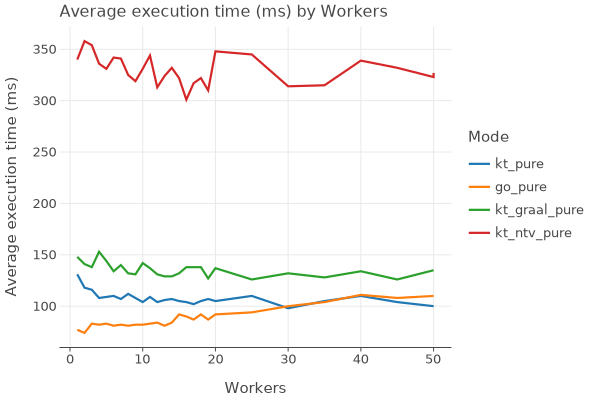
\includegraphics[width=\textwidth]{img/graphs/fixed_size_pure}
		\caption{Fixed Size Analysis \texttt{PURE}}
	\end{minipage}\hfill
	\begin{minipage}{0.25\textwidth}
		We can see that \Kotlin native incredibly suffers with the pure variant, showing that the native compilation is not optimized with channels communication. Instead, the \texttt{JVM} seems to have a good optimization of the message-passing technology. 
	\end{minipage}
\end{figure}

\subsubsection{Fixed workers}

\begin{figure}[H]
	\centering
	\begin{minipage}{0.7\textwidth}
		\centering
		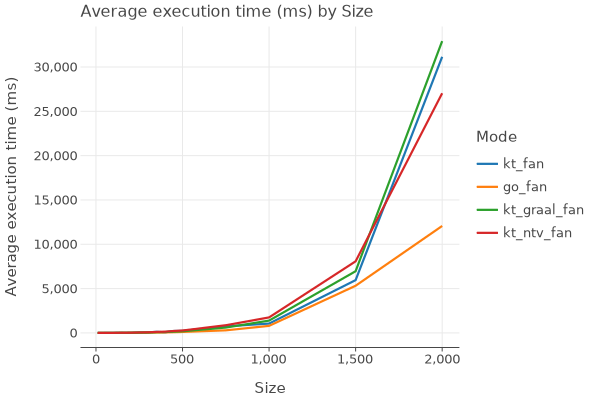
\includegraphics[width=\textwidth]{img/graphs/fixed_workers_fan}
		\caption{Fixed Workers Analysis \texttt{FAN}}
	\end{minipage}\hfill
	\begin{minipage}{0.25\textwidth}
		\Go keeps to be the one with the minimum elapsed times, while \texttt{Graal} shows some worsening especially with the increasing of the size.
	\end{minipage}
\end{figure}

\begin{figure}[H]
	\centering
	\begin{minipage}{0.7\textwidth}
		\centering
		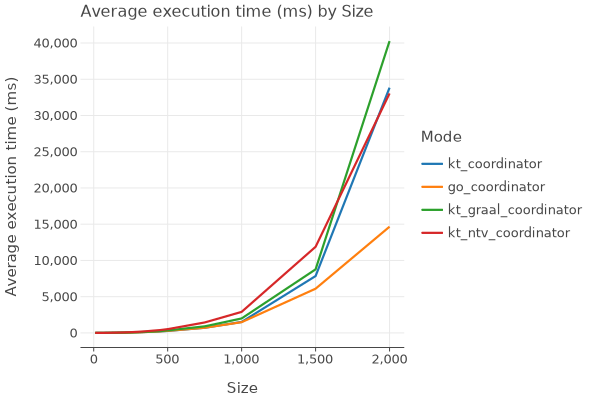
\includegraphics[width=\textwidth]{img/graphs/fixed_workers_coordinator}
		\caption{Fixed Workers Analysis  \texttt{COORDINATOR}}
	\end{minipage}\hfill
	\begin{minipage}{0.25\textwidth}
		The graphs is really similar to the previous one, with \Go as the best, \texttt{Graal} that suffers when the size increases while \Kotlin Native seems to recover some points at the end.
	\end{minipage}
\end{figure}

\begin{figure}[H]
	\centering
	\begin{minipage}{0.7\textwidth}
		\centering
		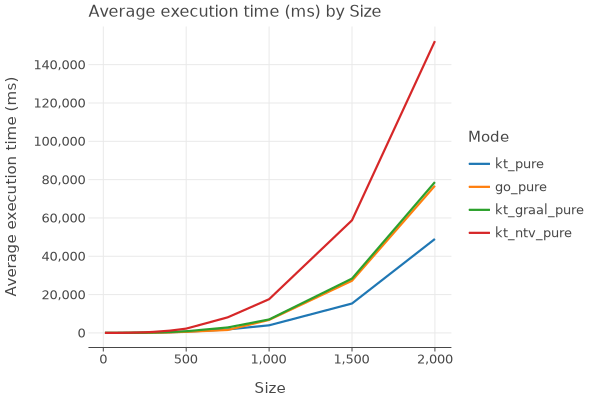
\includegraphics[width=\textwidth]{img/graphs/fixed_workers_pure}
		\caption{Fixed Workers Analysis \texttt{PURE}}
	\end{minipage}\hfill
	\begin{minipage}{0.25\textwidth}
		This graph shows some improvements for the \texttt{JVM} while \texttt{Graal} and \Go behave really similar. \Kotlin Native keeps to be the worst.
	\end{minipage}
\end{figure}

\subsection{The behavior of the \texttt{JVM} with multiple executions}

One of the reason why the coroutines have success on the \texttt{JVM}, is because they let to pay the cost of the Thread's creation only once. Then, since the Threads remains active and the coroutines are scheduled across them, the \texttt{JVM} does not have to loose time managin activation or de-activation of the them, saving lots of time.

This can be seen zooming into one of the \texttt{csv}, focusing on \Kotlin \texttt{JVM}:

\begin{lstlisting}
	workspaceId,size,coroutine,mode,timeMillis
	612f53a2-3b8b-4e39-84ee-0ee64bf1c89e,250,1,kt_coordinator,272
	612f53a2-3b8b-4e39-84ee-0ee64bf1c89e,250,1,kt_coordinator,102
	612f53a2-3b8b-4e39-84ee-0ee64bf1c89e,250,1,kt_coordinator,96
	612f53a2-3b8b-4e39-84ee-0ee64bf1c89e,250,1,kt_coordinator,89
	612f53a2-3b8b-4e39-84ee-0ee64bf1c89e,250,1,kt_coordinator,86
	612f53a2-3b8b-4e39-84ee-0ee64bf1c89e,250,1,kt_coordinator,80
	612f53a2-3b8b-4e39-84ee-0ee64bf1c89e,250,1,kt_coordinator,61
	612f53a2-3b8b-4e39-84ee-0ee64bf1c89e,250,1,kt_coordinator,61
	612f53a2-3b8b-4e39-84ee-0ee64bf1c89e,250,1,kt_coordinator,61
	612f53a2-3b8b-4e39-84ee-0ee64bf1c89e,250,1,kt_coordinator,61
\end{lstlisting}

\textbf{As we can see, the time of the first execution is almost 4.45 times the last one}. This is not happening on the compiled versions of \Go and \Kotlin Native, while the \texttt{Graal} show a significant improvement:

\begin{lstlisting}
	workspaceId,size,coroutine,mode,timeMillis
	324fbed9-a3a9-43af-b9be-add5ae409379,250,1,go_coordinator,48
	324fbed9-a3a9-43af-b9be-add5ae409379,250,1,go_coordinator,42
	324fbed9-a3a9-43af-b9be-add5ae409379,250,1,go_coordinator,48
	324fbed9-a3a9-43af-b9be-add5ae409379,250,1,go_coordinator,49
	324fbed9-a3a9-43af-b9be-add5ae409379,250,1,go_coordinator,47
	324fbed9-a3a9-43af-b9be-add5ae409379,250,1,go_coordinator,45
	324fbed9-a3a9-43af-b9be-add5ae409379,250,1,go_coordinator,44
	324fbed9-a3a9-43af-b9be-add5ae409379,250,1,go_coordinator,49
	324fbed9-a3a9-43af-b9be-add5ae409379,250,1,go_coordinator,42
	324fbed9-a3a9-43af-b9be-add5ae409379,250,1,go_coordinator,42
	ce8edcc7-1d94-427b-9d55-af4dbdd1d515,250,1,kt_graal_coordinator,132
	ce8edcc7-1d94-427b-9d55-af4dbdd1d515,250,1,kt_graal_coordinator,74
	ce8edcc7-1d94-427b-9d55-af4dbdd1d515,250,1,kt_graal_coordinator,76
	ce8edcc7-1d94-427b-9d55-af4dbdd1d515,250,1,kt_graal_coordinator,76
	ce8edcc7-1d94-427b-9d55-af4dbdd1d515,250,1,kt_graal_coordinator,76
	ce8edcc7-1d94-427b-9d55-af4dbdd1d515,250,1,kt_graal_coordinator,81
	ce8edcc7-1d94-427b-9d55-af4dbdd1d515,250,1,kt_graal_coordinator,76
	ce8edcc7-1d94-427b-9d55-af4dbdd1d515,250,1,kt_graal_coordinator,76
	ce8edcc7-1d94-427b-9d55-af4dbdd1d515,250,1,kt_graal_coordinator,81
	ce8edcc7-1d94-427b-9d55-af4dbdd1d515,250,1,kt_graal_coordinator,77
	727f-3326-faf8-efb0,250,1,kt_ntv_coordinator,132
	727f-3326-faf8-efb0,250,1,kt_ntv_coordinator,130
	727f-3326-faf8-efb0,250,1,kt_ntv_coordinator,169
	727f-3326-faf8-efb0,250,1,kt_ntv_coordinator,123
	727f-3326-faf8-efb0,250,1,kt_ntv_coordinator,124
	727f-3326-faf8-efb0,250,1,kt_ntv_coordinator,125
	727f-3326-faf8-efb0,250,1,kt_ntv_coordinator,126
	727f-3326-faf8-efb0,250,1,kt_ntv_coordinator,128
	727f-3326-faf8-efb0,250,1,kt_ntv_coordinator,126
	727f-3326-faf8-efb0,250,1,kt_ntv_coordinator,125
\end{lstlisting}

